\subsection{Sell Section}\label{subsec:manualsell}

To create a new auction you have to click on the Sell section on the top page
menu. You are redirected to a page where you have to fill out a form, writing
the name of the auction, the minimum bid and the minimum raise you accept for
that auction, the number of items you want to sell for this auction, the date
and time you want the auction to end and a description of the items. It is also
necessary to upload an image of the items for sale. Then, click on the button
``Sell''. If no errors are shown, you have created a new auction.

\begin{figure}[htb]
	\centering
	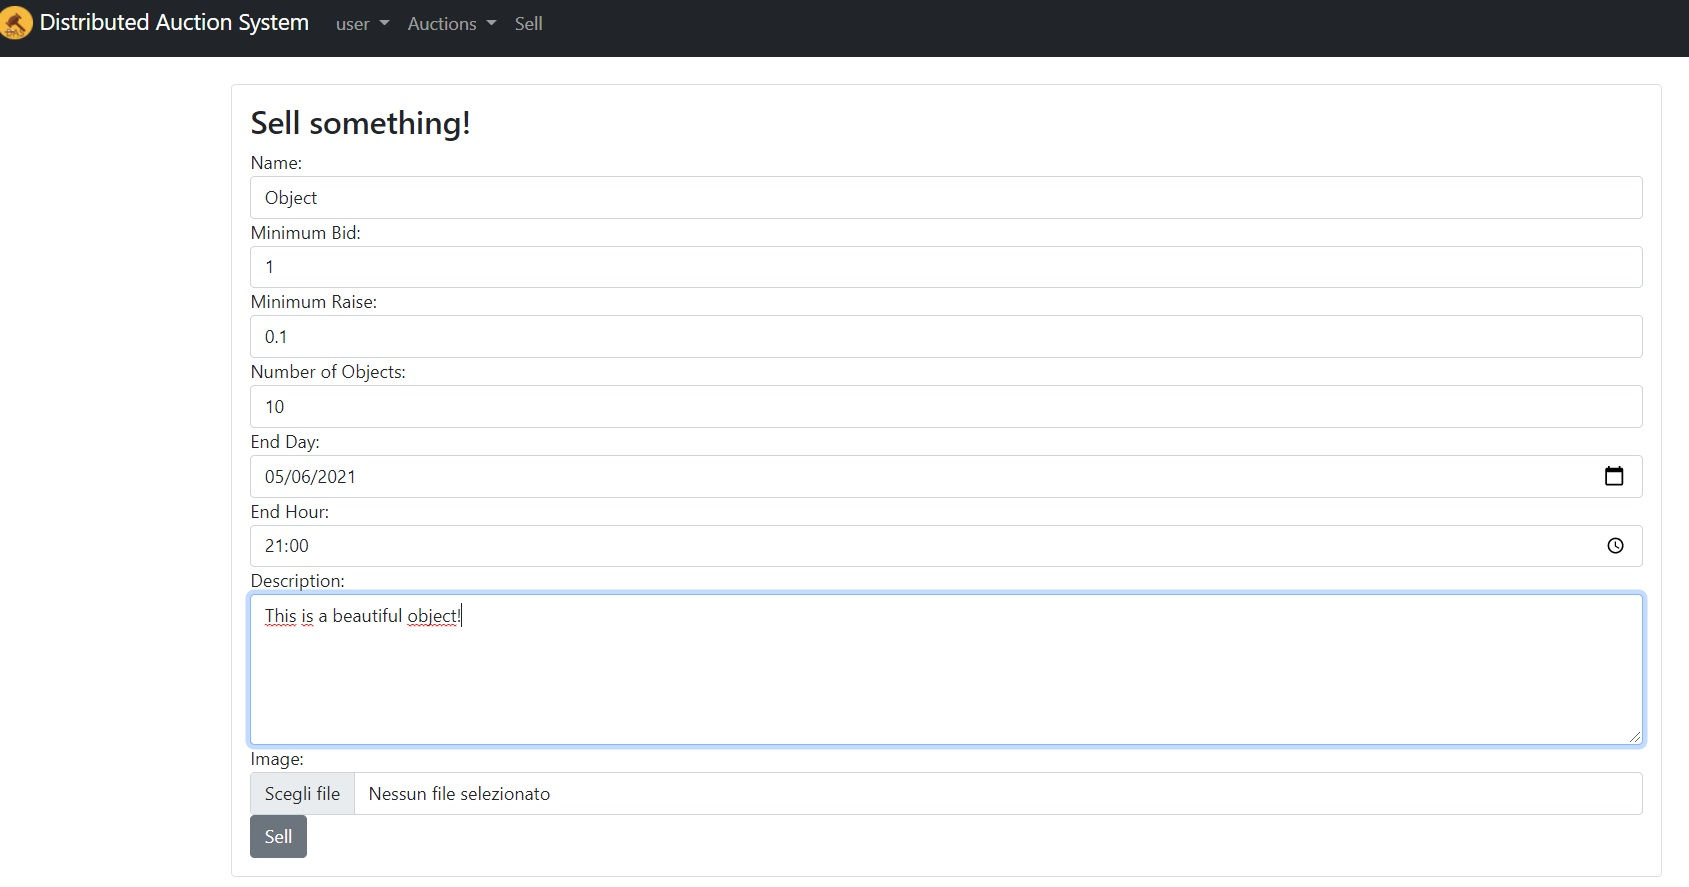
\includegraphics[width=\textwidth]{img/sell.jpg}
	\caption{Creation of a new auction}\label{fig:create-auction}
\end{figure}
